Over the past years, soft robotics have been a growing field of interest, as they have the potential to safely perform complex tasks in a human-centred environment. Besides executing tasks safely, the robot is demanded to be robust. Safety and robustness can be combined in the robotics design by considering material properties, locomotion, and morphology found in living organisms. Examples of bio-inspired soft robots include emulated trunks \cite{hannan2003kinematics} inspired by the proboscis of an elephant (Figure \ref{fig:BHA}), robots based on the arm of octopus \cite{wang2013visual}, or robots that replicate the movement of fish \cite{marchese2014autonomous}. These robots are created from soft and flexible materials, which ensures safe interaction with humans. However, they do have the necessary properties to grasp and pick-up objects. This flexibility theoretically gives the robot an infinite amount of degrees-of-freedom (DOFs). The robots redundancy gives rise to some advantages and challenges. One major advantage is, that a soft robot can exploit its redundancy to reach an end-effector position in multiple ways. Additionally, it enables the robot to grasp objects around obstacles more easily compared to rigid robots. Nevertheless, its theoretical infinite DOFs makes controlling these robotic systems more challenging as the robot is highly under-actuated. 

The main difference between soft robots and the well-known rigid robots is the robots' compliance \cite{trivedi2008soft}. Rigid robots generally consist of multiple rigid links that have mechanical actuators inside the joints. Each of this joint controls an additional DOF. A mechanical system is considered redundant if it has more degrees of freedom than those strictly required to execute a given task \cite{chiaverini2016redundant}. Opposed to rigid robots, bio-inspired robots do not necessarily have these links, and are therefore called continuum robots. Due to there continuous morphology, these robots are inherently redundant. Bio-inspired continuum robots can be classified into two categories namely, hard continuum robots and soft continuum robots. Hard continuum robots
generally consist of rigidly linked vertebrates that form the backbone of the soft robot. This backbone is compliant which results in a smooth deformation of the robot when external load is applied. An example is the elephant trunk's robot \cite{cieslak1999elephant}, which consists of eight elastic segments linked together by coil springs. Each segment has two pairs of strings that can control the movement of each individual segment. Servo or linear actuators can be use to wind and unwind the strings with that controlling the movement of the robot, these are so called tendon-driven robots. Soft continuum robots are generally composed of materials, whose mechanical strength is close to those of biological materials such as, muscles, skin, cartilage, and have a Young's modulus of around 1 gigapascal \cite{rus2015design}. Soft robots are generally pneumatically actuated, an example is the Bionic Handling Assistant (BHA) \cite{rolf2012constant} as shown in Figure \ref{fig:BHA}. By inflating chambers this robot is able to extend and bend. Soft robots are generally highly dexterous, which enables them grasp objects around obstacles. There are multiple challenges with regards to controlling soft robots. Due to its inherently flexible nature, heavy loads at the end-effector can cause deformation throughout the whole mechanical structure of the robot. Furthermore, the distributed body mass of the robot can have similar effects. This makes position sensing more difficult compared to a rigid manipulator, where forward kinematics can be easily formulated. Additionally, due to hyper-flexibility, multiple positions with the same end-effector position are possible, making the robot configuration for a given end-effector position non-unique.

\begin{figure}[H]
    \centering
    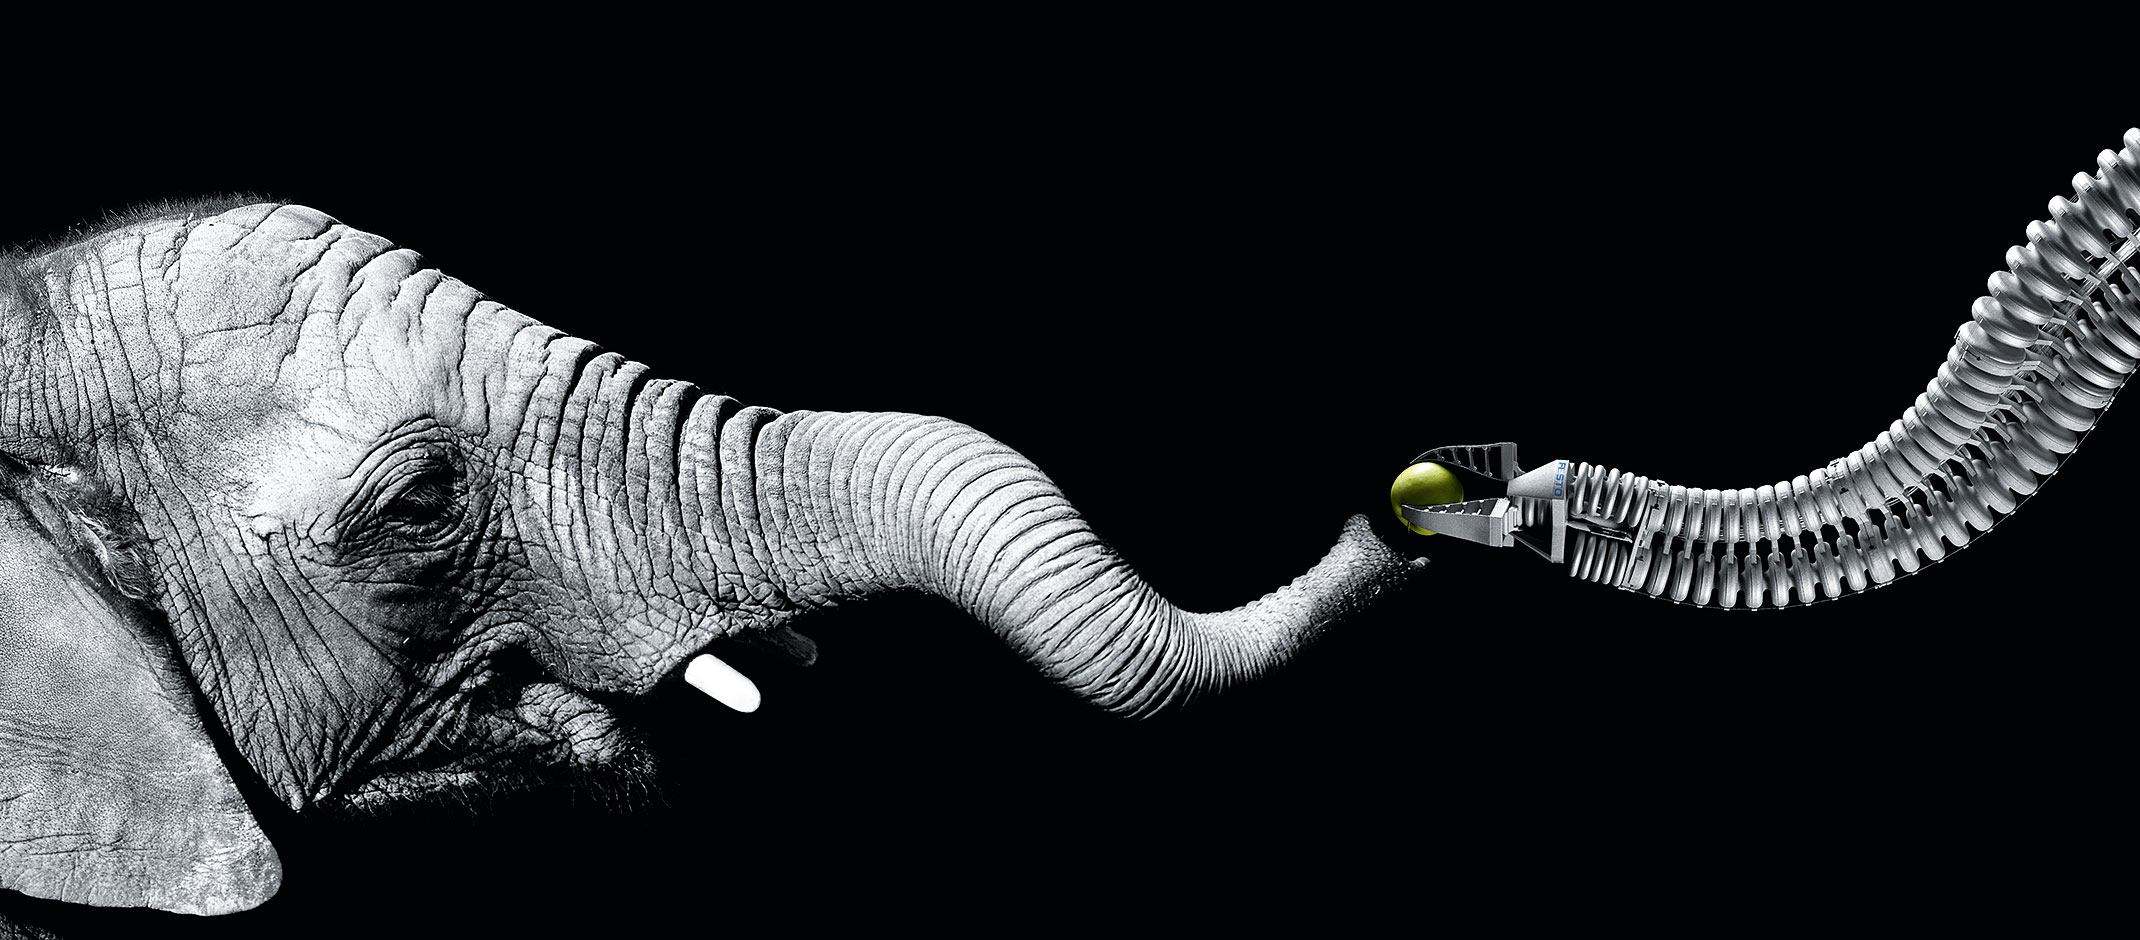
\includegraphics[width = \textwidth]{Figures/BHAelephant.jpg}
    \caption{Bionic Handling Assistant inspired by the trunk of an elephant \cite{BHA}.}
    \label{fig:BHA}
\end{figure}


  \begin{minipage}{\linewidth}
      \centering
      \begin{minipage}{0.45\linewidth}
          \begin{figure}[H]
              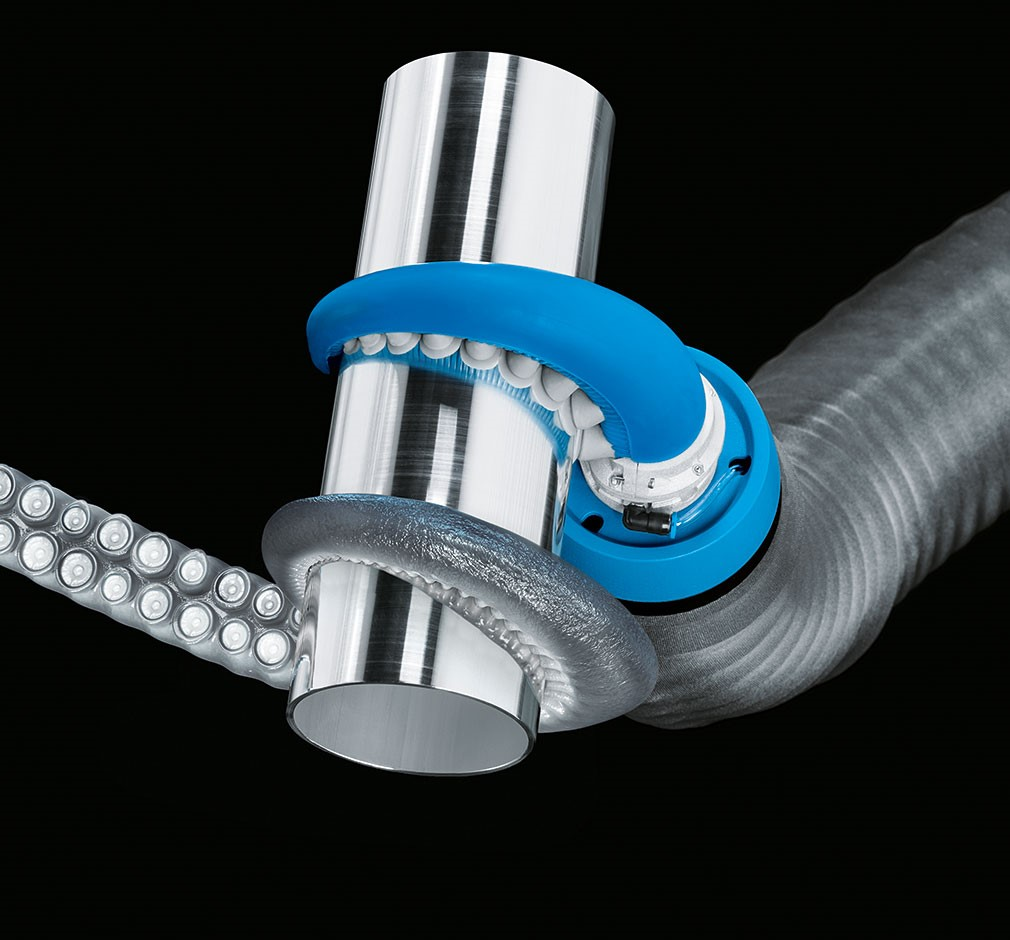
\includegraphics[width=\linewidth]{Figures/tentaclegripper (2).jpg}
              \caption{Octopus-inspired robot gripper able to move and manipulate a wide range of objects \cite{octopus}.}
          \end{figure}
      \end{minipage}
      \hspace{0.05\linewidth}
      \begin{minipage}{0.45\linewidth}
          \begin{figure}[H]
              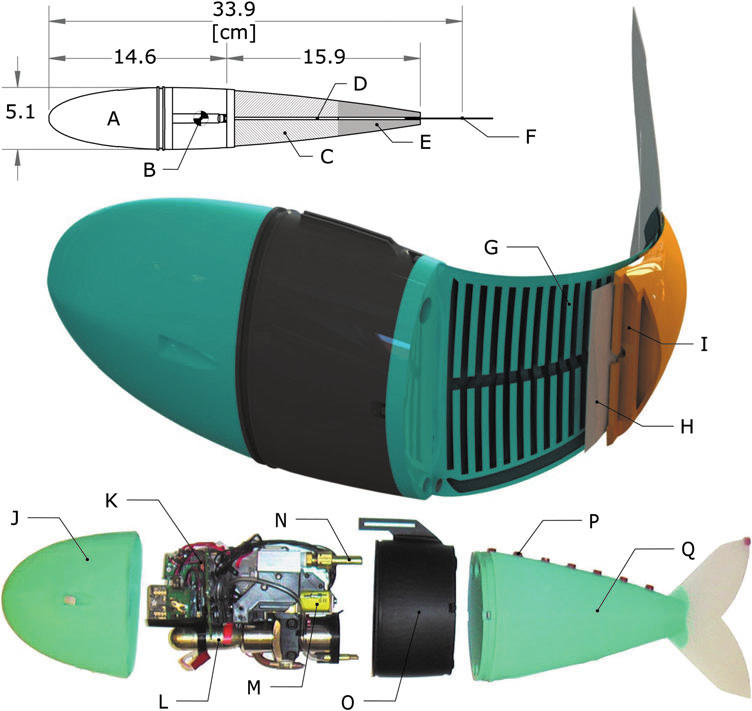
\includegraphics[width=\linewidth]{Figures/fish.jpg}
              \caption{Bio-inspired soft robot replicating movement of a fish \cite{marchese2014autonomous}.}
          \end{figure}
      \end{minipage}
  \end{minipage}

Thuruthel et al.(2018) \cite{george2018control} present an overview of soft robotic control for pneumatic actuated and tendon-driven soft robots. In this work, three control approaches can be distinguished, namely, model-free, hybrid and model-based control. For each control approach, a sub-division between kinematic and dynamical control is made. Here, kinematic control is defined as a zero order input-output relation. A change in input is directly observed in output, therefore this approach is lower-level compared to dynamical control. For the latter, the configuration space and/or task space variables velocities are used in the control algorithm. Model-free control does not use any kind of dynamical model in its control approach. Instead, it exploits learning-based algorithms to dynamically control the robotic system. This is the case for the work presented in \cite{rolf2013efficient}, where goal babbling is used to control the BHA. Goal babbling is defined as the ``bootstrapping of a coordination skill by repetitively trying to accomplish multiple goals related to that skill" \cite{rolf2012goal}. The goal of this control approach is to learn an inverse model, instead of feeding an inverse model directly to the algorithm. This inverse model is taught by using an exploring action, observing its outcomes and use the gathered data as a learning step. In \cite{reinhart2017hybrid}, a hybrid type of controller for the BHA was proposed. In this approach, a calculated inverse kinematic model is used together with a learning model. Previously, a model-based controller was used to control the BHA \cite{mahl2014bhakin}. However, this model-based controller only used a kinematic description of the soft robot. Later, a dynamic controller for the BHA was designed by \cite{falkenhahn2016dynamic}. This control approach used a cascaded controller formulation with a SISO controller to control individual bellow lengths, and inside a MIMO controller which features static gravity compensation, bending stiffness compensation,and dynamical interaction compensation. This method showed a significant improvement in the mobility of the BHA. The aforementioned examples illustrate that different control strategies can applied to the same robot configuration. 













%However, classic rigid robots still outperform the soft robots, in terms of accuracy, reputability, and speed. Soft robots theoretically have an infinite amount of degrees of freedom (DOF). However, the amount of actuators is limited. Hence, soft robots belong to the class of under actuated mechanical systems. This under actuation enables soft robots to reach a point in space in multiple ways, and grasp objects around obstacles. (cite de paper met figuren van soft robots die om een paal moeten grijpen) However, controlling under actuated systems has proven to be more difficult compared to fully actuated systems, where each degree of freedom is constrained by an actuator (bron). In this graduation project, we aim to improve the performance of a soft robot, by introducing an energy based control strategy. Our goal is to design a tracking controller, which is capable of pick and place tasks. This energy based control approach has, as far as we are concerned, not been applied in the field of soft robotics yet. This report has the following build up. First, recent research on dynamic modeling and control of soft robots will be presented. Then, conducted research on classic rigid robotics is shown. Here, we try to bridge the gap between control theory used for rigid robots and apply this theory to our soft robot. 

%\todo{maybe change the "energy based method" to a "model-based" control strategy, to not put the focus on one strategy directly and keep other options open}



%Several papers have been published on the control of soft robots, however most of them focus on inverse kinematic control. In \cite{reinhart2016hybrid}, inverse kinematic control of the Bionic Handling Assistant (BHA) designed by Festo is presented. This robot is pneumatically actuated and shows a lot of resemblances with the robot in the DC lab. The paper shows that feed-forward control based on inversion of a hybrid forward model. This hybrid model consists of two parts, an inverse kinematic part and a machine learning part. A constant curvature approach was used to model the robot, as presented in \cite{rolf2012constant}. Two learning algorithm are used: Linear Model and Extreme Learning Machine. In an earlier paper (\cite{queisser2014active}), an inverted equilibrium model of the same BHA was presented. These papers only propose kinematic control of the soft robot, whereas our aim is to develop a dynamic control algorithm. 

%\todo{other paper with learning control}


%Instead of using a learning element, visual based types of control have been control. Again, the control is based upon an inverse kinematic model. In  \cite{wang2013visual}, a cable-driven soft robotic manipulator is presented. This manipulator has a tentacle like shape, as its diameter decreases when moving away from its earths connection point. In total 4-cables are present inside the robots soft material, which can be used to control the manipulator. A piece wise constant curvature model is used to describe the kinematics of the manipulator, following the theory of (citeer een paper over CC model). A camera is fixed at the tip of the manipulator and a feature point is is fixed in 3D space around the robot. The camera is used to obtain a depth independent (2D) image Jacobian matrix. For controlling the system this depth-independent image Jacobian matrix, a PD-controller and gravity compensation is used to move the robot to its desired final position. This is done, by constantly estimating the depth-independent image Jacobian matrix. 















